% !TeX spellcheck = it_IT
\newpage
\section{Quantum computing}
Il quantum computing permette di risolvere una classe di problemi leggermente più ampia dei computer classici.
\begin{center}
	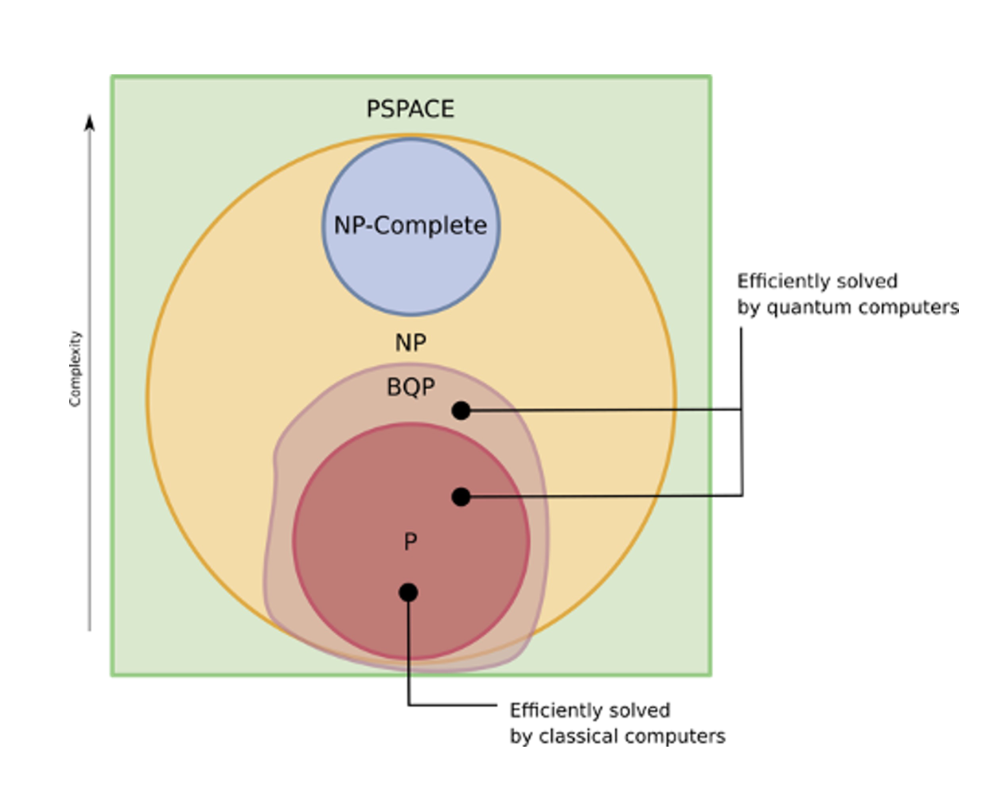
\includegraphics[scale=0.3]{quantum_problems.png}
\end{center}
Inoltre permette di risolvere problemi già risolvibili molto più velocemente. Ad esempio la ricerca di Grover in $O(\sqrt{n})$ invece che $O(n)$.

\subsection{Principi}
Un computer quantistico si basa su due proprietà della meccanica quantistica, \textbf{entaglement} e \textbf{superposizione}, per fornire un nuovo modo di rappresentare i dati, i \textbf{Qubits}, in modo da poterli elaborare in maniera più vantaggiosa.
\begin{definition}[Qubit]
	Un Qubit è una combinazione lineare di valori complessi dei due possibili stati base:
	\begin{itemize}
		\item \textit{Ground state}, $0$
		\item \textit{Excited state}, $1$
	\end{itemize}
	\begin{equation}
		\lvert \Psi \rangle = \alpha \lvert 0 \rangle + \beta \lvert 1 \rangle
	\end{equation}
\end{definition}
Concettualmente il Qubit è l'unità fondamentale di informazione quantistica che può assumere un valore pari a $0$, $1$ o una \textbf{superposizione}, ovvero una combinazione lineare dei due.\\
Quando poi viene osservato, il qubit collasserà ad uno dei due stati base con diverse probabilità in base alla sua superposizione.\\
Ne esistono vari tipi, ognuno con le sue caratteristiche.

\begin{definition}[Entaglement]
	Due Qubits sono entagled quando lo stato di uno è direttamente correlato con lo stato dell'altro, indipendentemente dalla loro distanza.
\end{definition}
\subsection{Programmazione}
L'idea è quindi di creare circuiti di Qubits che restituiscono un output di tipo probabilistico. Dato che al momento dell'osservazione la superposizione collassa ad un unico valore, per ottenere un risultato dobbiamo fare diverse iterazioni in modo da calcolare una probabilità.
\subsubsection{NISQ}
Al momento i computer quantistici sono di tipo \textbf{Noise Intermediate Scale Quantum}, ovvero molto sensibili alle interferenze e difficili da scalare. Questo implica che i programmi eseguibili al momento devono avere un piccolo numero di qubits e di operazioni.
\subsubsection{Quantum Software Engineering}
Un modo per superare le limitazioni dei computer quantistici attuali è combinando questi con i computer classici. Ad esempio tramite un \textbf{broker} che suddivida il lavoro in diversi pezzi e li distribuisca tra più macchine quantistiche, per poi alla fine recuperare tutti i risultati e combinarli.